\documentclass[SSS_Laborbericht.tex]{subfiles}
\usepackage{pdfpages}
\usepackage{listings}

\begin{document}

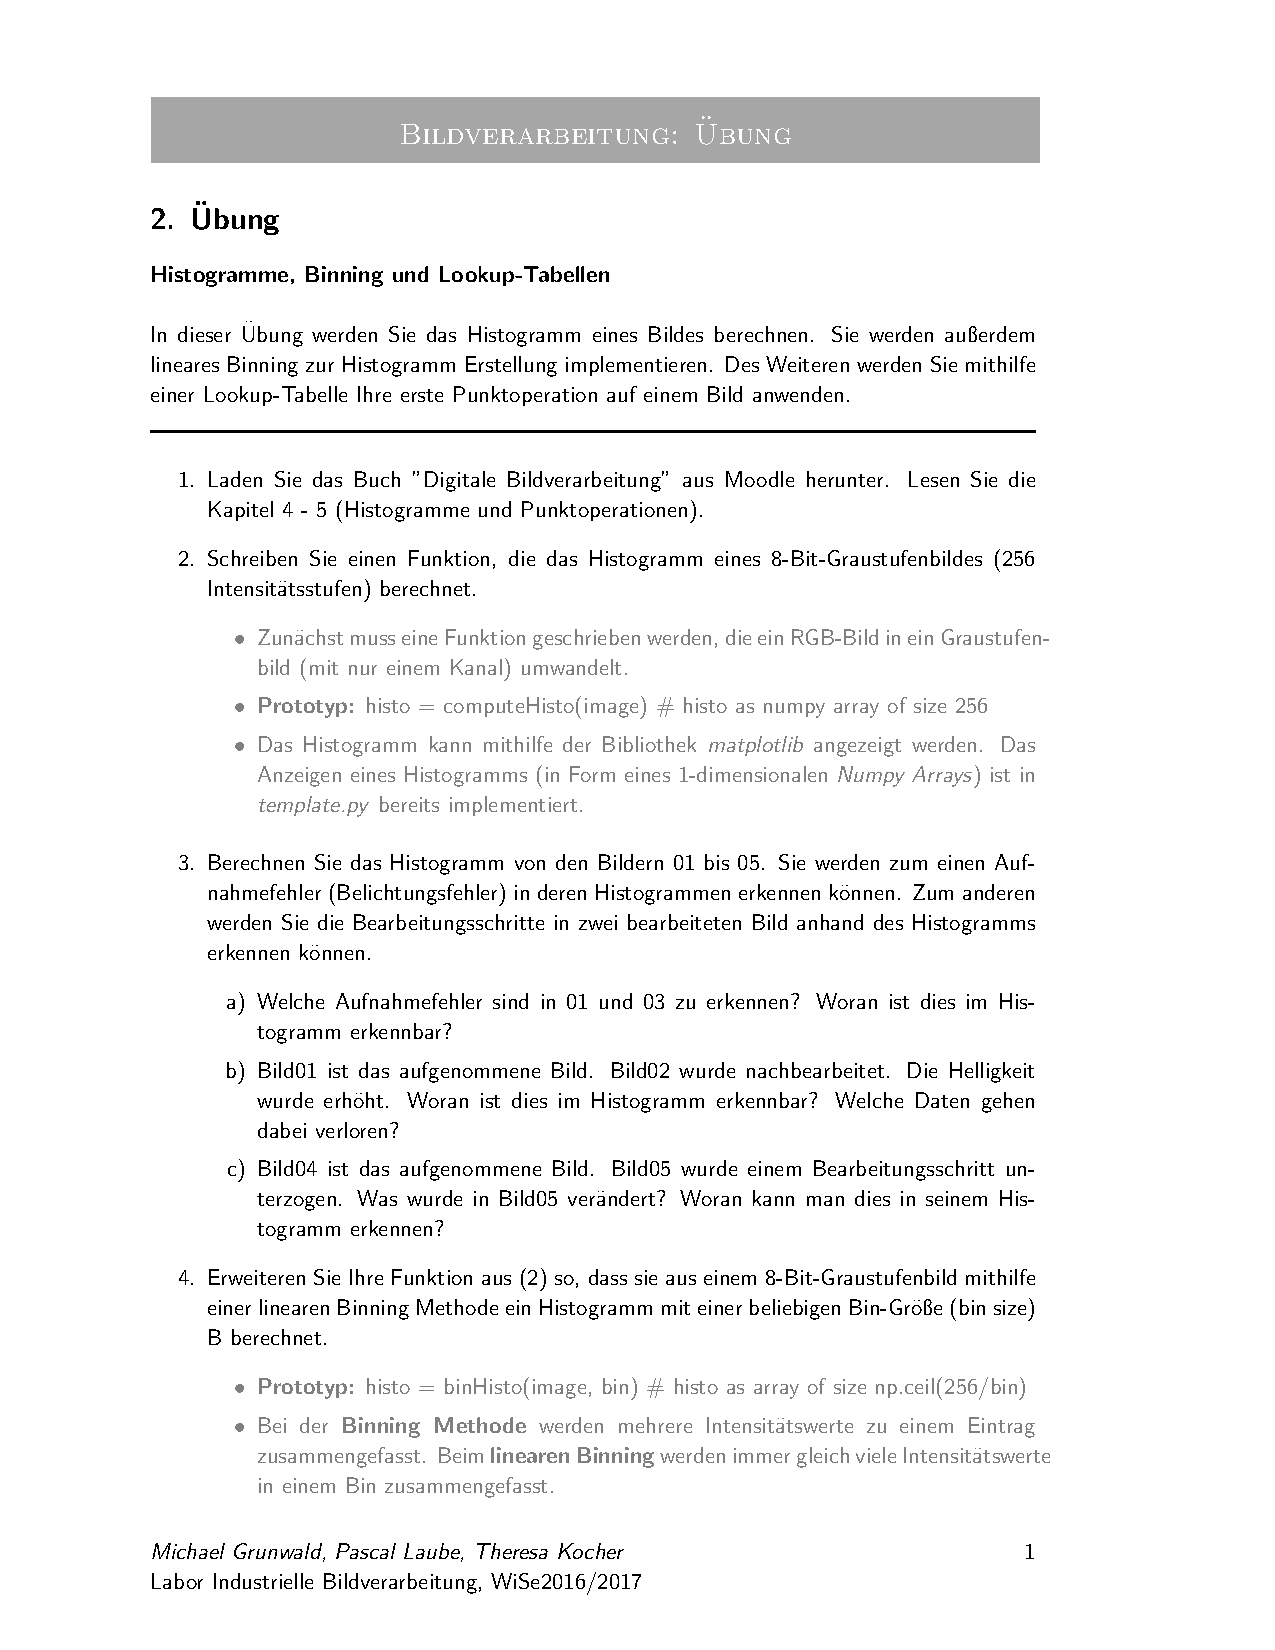
\includepdf[pages={1}]{uebung2.pdf}
\includepdf[pages={2}]{uebung2.pdf}

\noindent\Large{Aufgabe 2}
\lstinputlisting[style=PYTHON, frame=single, caption=rgb2gray, firstline=72, lastline=74, firstnumber=72]{template.py}

\lstinputlisting[style=PYTHON, frame=single, caption=rgb2gray, firstline=8, lastline=18, firstnumber=8]{template.py}

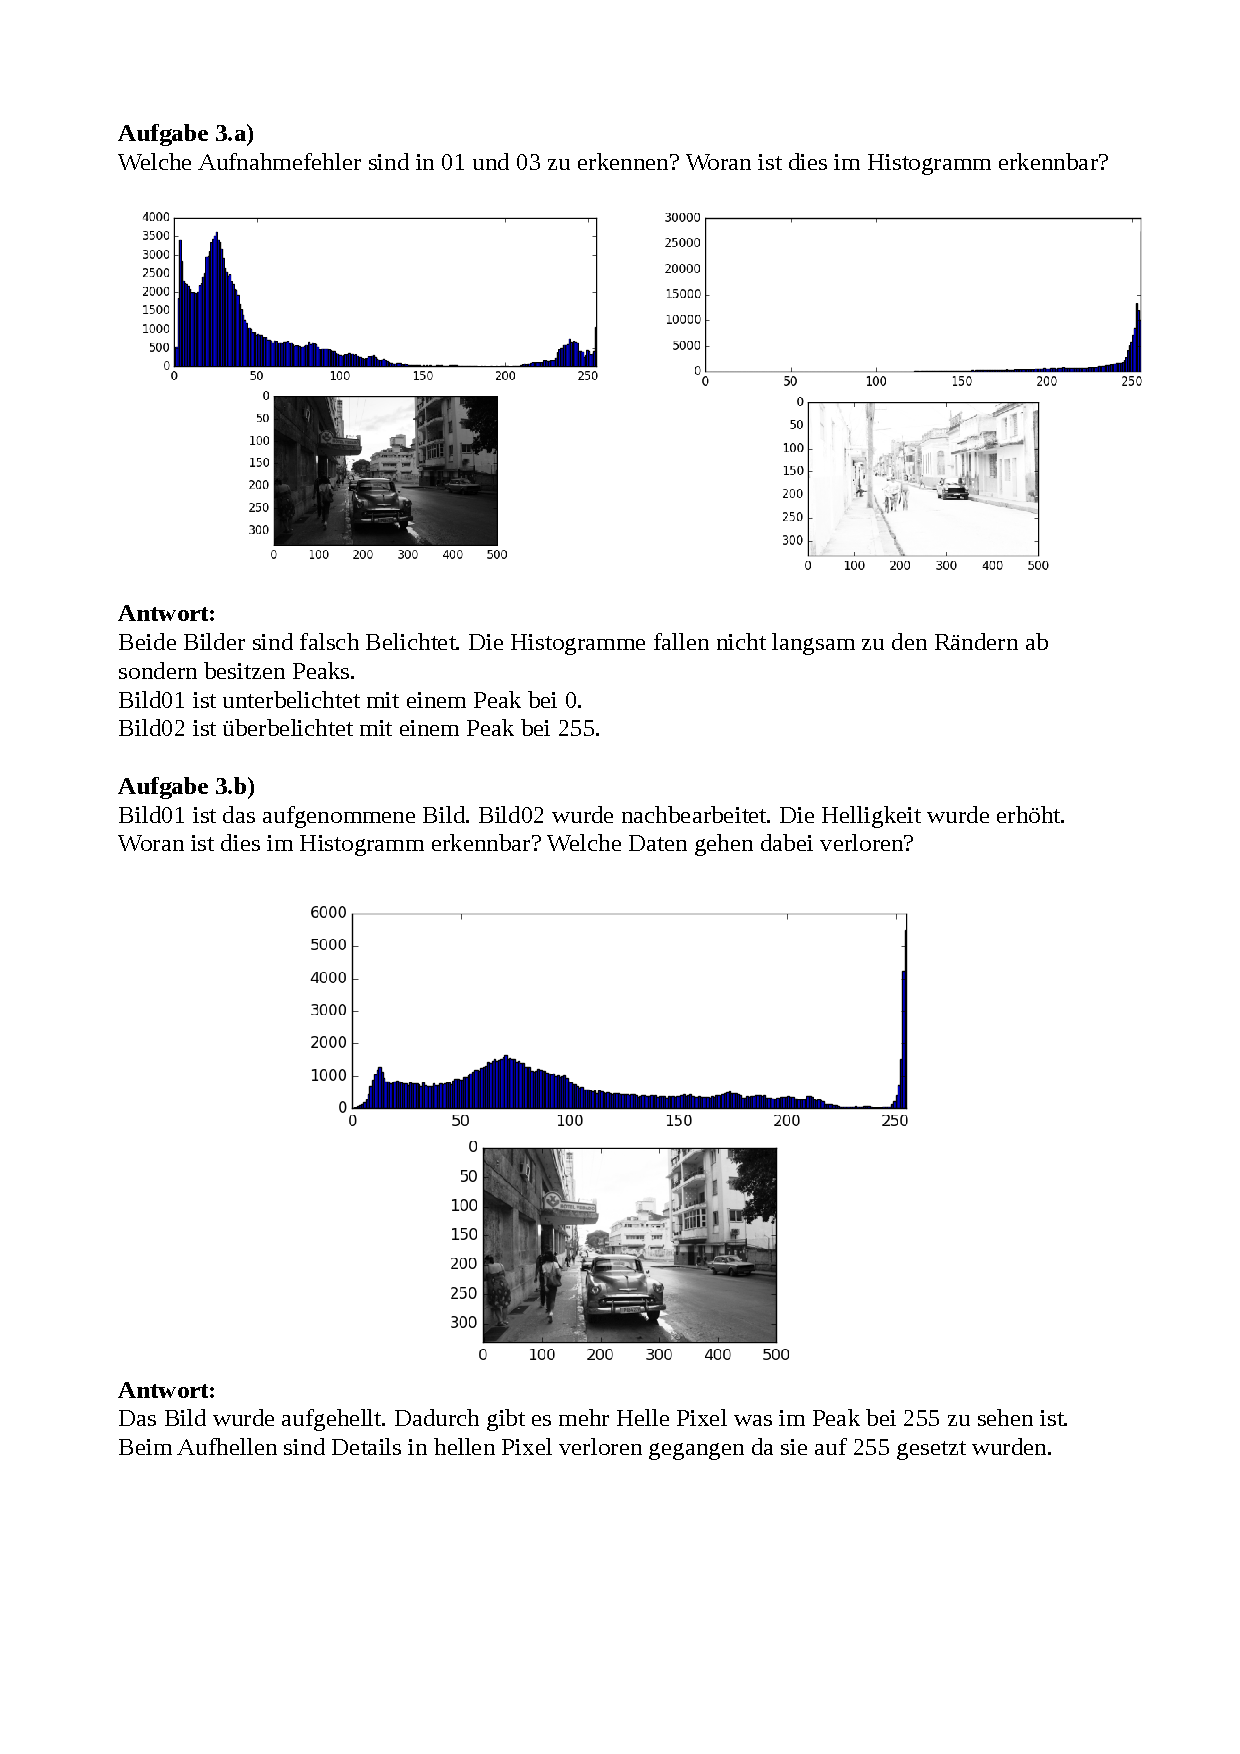
\includepdf[pages={1}]{Aufgabe3.pdf}
\includepdf[pages={2}]{Aufgabe3.pdf}

\noindent\Large{Aufgabe 4}
\lstinputlisting[style=PYTHON, frame=single, caption=rgb2gray, firstline=20, lastline=30, firstnumber=20]{template.py}

\newpage
\noindent\Large{Aufgabe 5.a)}
\noindent\normalsize{Wenn in einem Foto nur dunkle Bereich aufgehellt und helle Bereiche abgedunkelt werden können Details erhalten bleiben.}

\lstinputlisting[style=PYTHON, frame=single, caption=rgb2gray, firstline=33, lastline=69, firstnumber=33]{template.py}

\end{document}